\documentclass[12pt,a4paper]{article}
\usepackage[top=16mm,bottom=18mm,left=16mm,right=16mm,headheight=0pt,headsep=0mm,footskip=10mm]{geometry}
\usepackage{iftex}
\ifPDFTeX
  \usepackage[utf8]{inputenc}
  \usepackage[T5]{fontenc}
  \usepackage{mathptmx}
\else
  \usepackage{fontspec}
  \usepackage{mathptmx}
  \setmainfont{Times New Roman}
\fi
\usepackage{amsmath,amssymb}
\usepackage{xcolor}
\usepackage{tikz}
\usepackage{graphicx}
\usepackage{array,tabularx}
\usepackage{enumitem}
\usepackage{fancyhdr}
\usepackage{lastpage}

\definecolor{questionpurple}{RGB}{137,38,143}
\definecolor{answerblue}{RGB}{35,45,140}

\setlength{\parindent}{0pt}
\setlength{\parskip}{0pt}
\renewcommand{\baselinestretch}{1.12}
\pagestyle{fancy}
\fancyhf{}
\renewcommand{\headrulewidth}{0pt}
\fancyfoot[L]{\small Chuyên đề I -- Toán 11}
\fancyfoot[R]{\small Trang \thepage/\pageref{LastPage} -- Đề test số 01}
\renewcommand{\footrulewidth}{.4pt}

\newlist{questions}{enumerate}{1}
\setlist[questions]{label=\textcolor{questionpurple}{\bfseries Câu \arabic*.},leftmargin=0pt,itemindent=16mm,labelwidth=14mm,labelsep=2mm,align=left,itemsep=11pt,topsep=7pt,parsep=0pt}
\newcommand{\answerlabel}[1]{\tikz[baseline=(choice.base)]\node[draw=black!65,text=answerblue,circle,inner sep=0pt,minimum size=4.8mm,line width=.4pt,font=\normalsize] (choice) {#1};}
\newcommand{\fourchoices}[4]{\par\begingroup\setlength{\tabcolsep}{0pt}\renewcommand{\arraystretch}{1.35}\begin{tabularx}{\linewidth}{@{}*{4}{>{\raggedright\arraybackslash}X}@{}}\answerlabel{A}~#1 & \answerlabel{B}~#2 & \answerlabel{C}~#3 & \answerlabel{D}~#4\end{tabularx}\endgroup}
\newcommand{\twochoices}[4]{\par\begingroup\setlength{\tabcolsep}{0pt}\renewcommand{\arraystretch}{1.5}\begin{tabularx}{\linewidth}{@{}*{2}{>{\raggedright\arraybackslash}X}@{}}\answerlabel{A}~#1 & \answerlabel{B}~#2 \\ \answerlabel{C}~#3 & \answerlabel{D}~#4\end{tabularx}\endgroup}
\newcommand{\sd}{\mathop{\text{sđ}}\nolimits}

\begin{document}

\noindent
\begin{minipage}[t]{.35\textwidth}
  \centering
  {\bfseries CHUYÊN ĐỀ I -- TOÁN -- 11\par}
  \vspace{2pt}
  \rule{.72\linewidth}{.4pt}\par
  \vspace{3pt}
  CHƯƠNG I\par
  \vspace{4pt}
  {\itshape ĐỀ TEST SỐ 01\par}
\end{minipage}\hfill
\begin{minipage}[t]{.62\textwidth}
  \centering
  {\bfseries HÀM SỐ LƯỢNG GIÁC\par
  VÀ PHƯƠNG TRÌNH LƯỢNG GIÁC\par}
  \vspace{5pt}
  {\small\bfseries BÀI 1. GIÁ TRỊ LƯỢNG GIÁC\par
  CỦA GÓC LƯỢNG GIÁC\par}
\end{minipage}

\vspace{7mm}
\noindent
\begin{minipage}[t]{.72\textwidth}
  \textbf{Họ, tên thí sinh:}\dotfill\par
  \vspace{3pt}
  \textbf{Số báo danh:}\dotfill
\end{minipage}\hfill
\begin{minipage}[t]{.25\textwidth}
  \raggedleft
  \setlength{\fboxsep}{4pt}
  \fbox{\textbf{Đề test số: 01}}
\end{minipage}

\vspace{5mm}
\textbf{PHẦN I. Câu trắc nghiệm nhiều phương án lựa chọn.} Thí sinh trả lời từ câu 1 đến câu 12. Mỗi câu hỏi thí sinh chỉ chọn một phương án.

\begin{questions}
  \item Cho góc hình học $uOv$ có số đo $50^\circ$ (hình vẽ). Xác định số đo của các góc lượng giác $(Ou;Ov)$.

  \begin{center}
  \begin{tikzpicture}[scale=1.05]
    \draw[black,line width=.8pt] (0,0) -- (3.2,0) node[below,text=black] {$u$};
    \draw[black,line width=.8pt] (0,0) -- (50:3.2) node[above left,text=black] {$v$};
    \draw[black,line width=.6pt] (1.15,0) arc[start angle=0,end angle=50,radius=1.15];
    \node at (25:1.55) {$50^\circ$};
    \node[below left] at (0,0) {$O$};
  \end{tikzpicture}
  \end{center}
  \twochoices
    {$\sd (Ou;Ov)=50^\circ+k360^\circ, k\in\mathbb{Z}$.}
    {$\sd (Ou;Ov)=50^\circ+k180^\circ, k\in\mathbb{Z}$.}
    {$\sd (Ou;Ov)=-50^\circ+k360^\circ, k\in\mathbb{Z}$.}
    {$\sd (Ou;Ov)=-50^\circ+k180^\circ, k\in\mathbb{Z}$.}

  \item Bánh xe của người đi xe đạp quay được 2 vòng trong 6 giây. Hỏi trong 1 giây, bánh xe quay được bao nhiêu độ:
  \fourchoices{$60^\circ$.}{$72^\circ$.}{$240^\circ$.}{$120^\circ$.}

  \item Cho góc lượng giác $(Ou,Ov)$ có số đo là $\dfrac{\pi}{4}$. Số đo của góc lượng giác nào sau đây có cùng tia đầu là $Ou$ và tia cuối là $Ov$?
  \fourchoices{$\dfrac{3\pi}{4}$.}{$\dfrac{17\pi}{4}$.}{$\dfrac{7\pi}{4}$.}{$\dfrac{5\pi}{4}$.}

  \item Đổi số đo góc $105^\circ$ sang rađian, ta được
  \fourchoices{$\dfrac{5\pi}{12}\,rad$.}{$\dfrac{7\pi}{12}\,rad$.}{$\dfrac{9\pi}{12}\,rad$.}{$\dfrac{5\pi}{8}\,rad$.}

  \item Cho góc $\alpha$ thỏa mãn $0<\alpha<\dfrac{\pi}{2}$ và $\cos\alpha=\dfrac{1}{3}$. Tính $\sin\alpha$.
  \fourchoices{$\dfrac{-2\sqrt{2}}{3}$.}{$\dfrac{2\sqrt{2}}{3}$.}{$\dfrac{-\sqrt{2}}{3}$.}{$\dfrac{\sqrt{2}}{3}$.}

  \item Bánh xe của người đi xe đạp quay được 13 vòng trong 4 giây. Tính độ dài quãng đường mà người đi xe đạp đã đi được trong 2 phút, biết rằng đường kính của bánh xe đạp là $580\,mm$, lấy $\pi\approx 3{,}14$.
  \fourchoices{$710{,}6283\ (km)$.}{$1421{,}2565\ (m)$.}{$710{,}6283\ (m)$.}{$1421{,}2565\ (km)$.}
\end{questions}

\newpage

\begin{center}
  {\small\bfseries\itshape CHUYÊN ĐỀ I -- TOÁN -- 11 -- HÀM SỐ LƯỢNG GIÁC VÀ PHƯƠNG TRÌNH LƯỢNG GIÁC}
\end{center}

\begin{questions}[resume,itemsep=7pt,topsep=3pt]
  \item
  \begin{minipage}[t]{\dimexpr.60\linewidth-16mm\relax}
    Trên đường tròn lượng giác, số đo của các góc lượng giác có tia đầu $OA$, tia cuối $OB$ là
    \par\vspace{5mm}
    \twochoices
      {$\dfrac{\pi}{2}+k\pi, k\in\mathbb{Z}$.}
      {$\dfrac{\pi}{4}+k2\pi, k\in\mathbb{Z}$.}
      {$-\dfrac{\pi}{2}+k2\pi, k\in\mathbb{Z}$.}
      {$\dfrac{\pi}{2}+2k\pi, k\in\mathbb{Z}$}
  \end{minipage}\hfill
  \begin{minipage}[t]{.38\linewidth}
    \vspace{0pt}
    \centering
    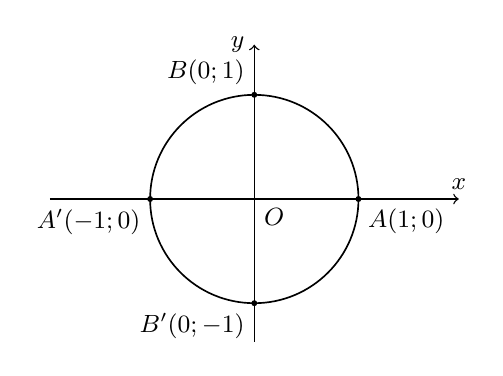
\begin{tikzpicture}[scale=.98,font=\small]
      \draw[line width=.6pt] (0,0) circle (1.35);
      \draw[->,line width=.5pt] (-2.65,0) -- (2.65,0) node[above] {$x$};
      \draw[->,line width=.5pt] (0,-1.85) -- (0,2) node[left] {$y$};
      \fill (1.35,0) circle (1.1pt) node[below right] {$A(1;0)$};
      \fill (-1.35,0) circle (1.1pt) node[below left] {$A'(-1;0)$};
      \fill (0,1.35) circle (1.1pt) node[above left] {$B(0;1)$};
      \fill (0,-1.35) circle (1.1pt) node[below left] {$B'(0;-1)$};
      \node[below right] at (0,0) {$O$};
    \end{tikzpicture}
  \end{minipage}

  \item Cho $\sin\alpha=\dfrac{4}{5}$ và $\dfrac{\pi}{2}<\alpha<\pi$. Tính $\cos\alpha$.
  \fourchoices{$\dfrac{3}{5}$.}{$\dfrac{1}{5}$.}{$-\dfrac{1}{5}$.}{$-\dfrac{3}{5}$.}

  \item Cho một góc lượng giác $(Ox,Ou)$ có số đo là $-120^\circ$ và một góc lượng giác $(Ox,Ov)$ có số đo $230^\circ$. Số đo của các góc lượng giác $(Ou,Ov)$ là:
  \twochoices
    {$\sd (Ou,Ov)=350^\circ+k\cdot360^\circ\ (k\in\mathbb{Z})$.}
    {$\sd (Ou,Ov)=110^\circ+k\cdot360^\circ\ (k\in\mathbb{Z})$.}
    {$\sd (Ou,Ov)=-350^\circ+k\cdot360^\circ\ (k\in\mathbb{Z})$.}
    {$\sd (Ou,Ov)=-110^\circ+k\cdot360^\circ\ (k\in\mathbb{Z})$.}

  \item Trên đường tròn bán kính $r=15$, độ dài của cung có số đo $\alpha=50^\circ$ là
  \fourchoices{$l=750$.}{$l=15\cdot\dfrac{180}{\pi}$.}{$l=\dfrac{15\pi}{180}$.}{$l=\dfrac{25\pi}{6}$.}

  \item Cho $\cos\alpha=\dfrac{2}{3}$ và $\alpha\in\left(\dfrac{3\pi}{2};2\pi\right)$. Tính $\cot\alpha$.
  \fourchoices{$\dfrac{2\sqrt{5}}{5}$.}{$-\dfrac{2\sqrt{5}}{5}$.}{$\dfrac{\sqrt{5}}{3}$.}{$-\dfrac{\sqrt{5}}{3}$.}

  \item Cho $\cos\alpha=\dfrac{3}{7}$ và $\dfrac{3\pi}{2}<\alpha<2\pi$. Khi đó $\sin\alpha$ bằng
  \fourchoices{$\dfrac{4}{7}$.}{$-\dfrac{4}{7}$.}{$-\dfrac{2\sqrt{10}}{7}$.}{$\dfrac{2\sqrt{10}}{7}$.}
\end{questions}

\vspace{4mm}
\textbf{PHẦN II. Câu trắc nghiệm đúng sai.} Thí sinh trả lời từ câu 1 đến câu 4. Trong mỗi ý a), b), c), d) ở mỗi câu, thí sinh chọn đúng hoặc sai.

\begin{questions}[start=1,topsep=4pt]
  \item Cho hình vẽ sau:
  \par\vspace{3mm}
  \begin{minipage}[t]{.64\linewidth}
    \vspace{0pt}
    \begin{enumerate}[label=\alph*),leftmargin=7mm,labelsep=1mm,itemsep=5pt,topsep=0pt,parsep=0pt]
      \item Số đo góc lượng giác $(OM,OA)$ là
      \par\vspace{3pt}
      $\sd(OM,OA)=\dfrac{\pi}{3}+k2\pi\ (k\in\mathbb{Z})$.
      \item $\sd(ON,OA)=\sd(ON,OM)-\sd(OA,OM)$.
      \item Độ dài cung tròn AM lớn là: $l_{AM}=\dfrac{2\pi}{3}$.
      \item Hai điểm $M,N$ biểu diễn các cung có số đo là:
      \par\vspace{3pt}
      $x=\dfrac{\pi}{3}+k\pi\ (k\in\mathbb{Z})$.
    \end{enumerate}
  \end{minipage}\hfill
  \begin{minipage}[t]{.33\linewidth}
    \vspace{0pt}
    \centering
    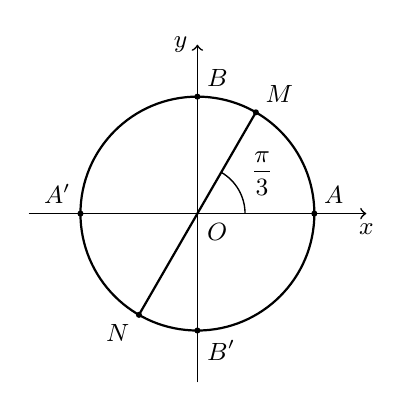
\begin{tikzpicture}[scale=1.1,font=\small]
      \draw[line width=.8pt] (0,0) circle (1.35);
      \draw[->,line width=.6pt] (-1.95,0) -- (1.95,0) node[below] {$x$};
      \draw[->,line width=.6pt] (0,-1.95) -- (0,1.95) node[left] {$y$};
      \draw[line width=.8pt] (240:1.35) -- (60:1.35);
      \draw[line width=.5pt] (.55,0) arc[start angle=0,end angle=60,radius=.55];
      \node at (32:.88) {$\dfrac{\pi}{3}$};
      \fill (1.35,0) circle (1pt) node[above right] {$A$};
      \fill (-1.35,0) circle (1pt) node[above left] {$A'$};
      \fill (0,1.35) circle (1pt) node[above right] {$B$};
      \fill (0,-1.35) circle (1pt) node[below right] {$B'$};
      \fill (60:1.35) circle (1pt) node[above right] {$M$};
      \fill (240:1.35) circle (1pt) node[below left] {$N$};
      \node[below right] at (0,0) {$O$};
    \end{tikzpicture}
  \end{minipage}
\end{questions}

\newpage

\begingroup
\renewcommand{\baselinestretch}{1.03}\selectfont
\begin{center}
  {\small\bfseries\itshape CHUYÊN ĐỀ I -- TOÁN -- 11 -- HÀM SỐ LƯỢNG GIÁC VÀ PHƯƠNG TRÌNH LƯỢNG GIÁC}
\end{center}

\begin{questions}[resume,itemsep=5pt,topsep=3pt]
  \item Cho góc lượng giác $\alpha$ có số đo theo đơn vị rađian là $\dfrac{3\pi}{4}$.
  \begin{enumerate}[label=\alph*),leftmargin=7mm,labelsep=1mm,itemsep=3pt,topsep=3pt,parsep=0pt]
    \item Góc lượng giác $\alpha$ có số đo theo đơn vị độ là $155^\circ$.
    \item Điểm biểu diễn góc lượng giác $\alpha$ là điểm $M$ trên đường tròn lượng giác thuộc góc phần tư thứ I.
    \item Góc lượng giác $-\dfrac{5\pi}{4}$ có cùng điểm biểu diễn trên đường tròn lượng giác với góc $\alpha$.
    \item Góc lượng giác $855^\circ$ có cùng điểm biểu diễn trên đường tròn lượng giác với góc $\alpha$.
  \end{enumerate}

  \item Cho góc $\alpha$ thỏa mãn $\cos\alpha=\dfrac{3}{5}$ và $-\dfrac{\pi}{2}<\alpha<0$.
  \begin{enumerate}[label=\alph*),leftmargin=7mm,labelsep=1mm,itemsep=3pt,topsep=3pt,parsep=0pt]
    \item $\sin\alpha>0$.
    \item $\tan\alpha<0$.
    \item $\sin\alpha=-\dfrac{4}{5}$.
    \item $\sin\left(\dfrac{\pi}{2}-\alpha\right)-\sin(-\alpha)=\dfrac{7}{5}$.
  \end{enumerate}

  \item Cho góc $\alpha$ $(0^\circ<\alpha<180^\circ)$ thỏa mãn $\tan\alpha=3$.
  \begin{enumerate}[label=\alph*),leftmargin=7mm,labelsep=1mm,itemsep=3pt,topsep=3pt,parsep=0pt]
    \item $\cot\alpha=\dfrac{1}{\sqrt{3}}$.
    \item $\cos\alpha>0$.
    \item $\sin\alpha=\dfrac{3\sqrt{10}}{10}$.
    \item $P=\dfrac{2\sin\alpha-3\cos\alpha}{3\sin\alpha+2\cos\alpha}=\dfrac{-3}{11}$.
  \end{enumerate}
\end{questions}

\vspace{3mm}
\textbf{PHẦN III. Câu trắc nghiệm trả lời ngắn.} Thí sinh trả lời từ câu 1 đến câu 6.

\begin{questions}[start=1,itemsep=5pt,topsep=5pt]
  \item Cho $\cos x=\dfrac{1}{3}$. Tính giá trị biểu thức $P=3\sin^2x+4\cos^2x$. (kết quả làm tròn đến hàng phần mười)

  \item Cho $\tan\alpha=2$, Giá trị biểu thức $P=\dfrac{4\sin\alpha+5\cos\alpha}{2\sin\alpha-3\cos\alpha}$ là

  \item Cho biết $\cot x=\dfrac{1}{2}$. Tính giá trị của biểu thức $A=\dfrac{2}{\sin^2x-\sin x\cdot\cos x-\cos^2x}$.

  \item Bánh xe đạp của người đi xe đạp quay được 2 vòng trong 5 giây. Hỏi trong 2 giây, bánh xe quay được 1 góc bao nhiêu rad (kết quả làm tròn đến hàng phần mười)?

  \item Một bánh xe đạp quay được 25 vòng trong 10 giây.
  \par\vspace{2mm}
  {\centering
    \includegraphics[width=53mm]{prism-uploads/{D7E6C55C-B4F1-4F32-A58C-ECC3EC349DC6}.png}\par
  }
  \vspace{2mm}
  Tính độ dài quãng đường mà người đi xe thực hiện được trong $2{,}35$ phút, biết rằng bán kính bánh xe bằng $340\,mm$. (Tính theo đơn vị mét, kết quả được làm tròn đến hàng đơn vị).
\end{questions}
\endgroup

\newpage

\begin{center}
  {\small\bfseries\itshape CHUYÊN ĐỀ I -- TOÁN -- 11 -- HÀM SỐ LƯỢNG GIÁC VÀ PHƯƠNG TRÌNH LƯỢNG GIÁC}
\end{center}

\begin{questions}[start=6,topsep=3pt]
  \item Một chiếc đu quay có bán kính $75\,m$, tâm của vòng quay ở độ cao $90\,m$ so với mặt đất, thời gian thực hiện mỗi vòng quay của đu quay là 30 phút. Nếu một người vào cabin tại vị trí thấp nhất của vòng quay, thì sau 20 phút quay, người đó ở độ cao bao nhiêu mét so với mặt đất?
  \par\vspace{4mm}
  {\centering
    \includegraphics[width=78mm]{prism-uploads/{109023E2-D2DC-4F76-A467-EC48233A3065}.png}\par
  }
\end{questions}

\vspace{5mm}
\begin{center}
  \textbf{---------- HẾT ----------}
\end{center}

\end{document}
